\chapter{Dangless - Implementation}
\label{ch:implementation}

\section{API overview}

Dangless is a Linux static library \texttt{libdangless.a} that can be linked to any application during build time. \todo{Probably should write about how to build it and how to link it to existing applications.} It defines a set of functions for allocating and deallocating memory:

\begin{lstlisting}
// sources/include/dangless/dangless_malloc.h

void *dangless_malloc(size_t sz) __attribute__((malloc));
void *dangless_calloc(size_t num, size_t size) __attribute__((malloc));
void *dangless_realloc(void *p, size_t new_size);
int dangless_posix_memalign(void **pp, size_t align, size_t size);
void dangless_free(void *p);
\end{lstlisting}

These functions have the exact same signature and behaviour as their standard counterparts \lstinline!malloc()!, \lstinline!calloc()!, and \lstinline!free()!. In fact, because the GNU C Library defines these standard functions as weak symbols~\cite{glibc-malloc-is-weak}, Dangless provides an option (\lstinline!CONFIG_OVERRIDE_SYMBOLS!) to override the symbols with its own implementation, enabling the user code to perform memory management without even being aware that it's using Dangless in the background.

Besides the above functions, Dangless defines a few more functions, out of which the following two are important.

\begin{lstlisting}
void dangless_init(void);
\end{lstlisting}

First, \lstinline!dangless_init()! initializes Dangless, and has to be called before any memory management is performed that Dangless should protect. The most important thing that this function does is initialize and enter Dune by calling \lstinline!dune_init()! and \lstinline!dune_enter()!. Dangless relies on Dune to be able to manipulate the page tables. Afterwards, we register our own pagefault handler with Dune, which enables us to detect when a memory access has failed due to the protection that Dangless offers.

By default, Dangless automatically registers this function in the \lstinline!.preinit_array! section of the binary, causing it to be called automatically before any user-defined constructors or the \lstinline!main()! entry point. This can be disabled via the \lstinline!CONFIG_REGISTER_PREINIT! option.

It's important to note that heap memory allocation can and does happen \emph{before} \lstinline!dangless_init()! is called, for example as part of the glibc runtime initialization. This case needs to be handled, so all of the \lstinline!dangless_! functions simply pass the call through to the underlying (system) allocator without doing anything else if they are called before \lstinline!dangless_init()!.

\begin{lstlisting}
int dangless_dedicate_vmem(void *start, void *end);
\end{lstlisting}

In order for Dangless to work, it requires exclusive use of some virtual memory to remap user allocations into. This region has to be large, as each \lstinline!dangless_malloc()! call will use up at least one page from it, and currently this virtual memory is never re-used because we lack a mechanism (such as a garbage collector) to be reasonably certain that a given virtual memory page is no longer referenced. This function can be used to make virtual memory regions available to Dangless for this purpose.

Since users of Dangless will typically not know or want to make this decision themselves, we provide the option \lstinline!CONFIG_AUTO_DEDICATE_MAX_PML4ES! which allows Dangless to take ownership of one or more unused PML4 pagetable entries which can each map 512 gigabytes of memory. This occurs at most once when a \lstinline!dangless_malloc()! or similar call is made, but Dangless does not have sufficient virtual memory available to it to protect the call.

This solution is very simplistic, and a smarter way to take ownership of virtual memory is decidedly possible. For instance, any time we require more virtual memory, we could scan the page tables and take ownership of some amount of currently-unused page table entries. Some implementation effort would need to be made to make sure this doesn't conflict with Dune's virtual memory allocation. However, this is very easy in the used Dune version, as Dune's page allocator (as defined in \texttt{libdune/dune.h}) uses maximum \lstinline!MAX_PAGES = (1 << 20)! pages (i.e. 4 GB of memory) starting at \lstinline!PAGEBASE = 0x200000000!. Any memory outside of this that is not used to hold application or kernel code or data is available for use by Dangless uncontested.

\section{Performing an allocation}

Whenever Dangless is asked to allocate some memory via a call to \lstinline!dangless_malloc()!, \lstinline!dangless_calloc()!, or \lstinline!dangless_realloc()!, a number of steps have to happen: physical memory has to be allocated, virtual memory has to be allocated, and the mapping created. Most of the process is the same regardless of the exact function called. The only exception is \lstinline!dangless_realloc()!, which I will detail later.

\subsection{Allocating physical memory}

The first step Dangelss has to perform is to acquire the physical memory it can use to satisfy the allocation. It does not currently defer allocating physical memory like kernels typically do, although in principle it could.
Since the goal of Dangless is only to provide security benefits, Dangless has no strategy of physical memory management unlike normal implementations. In fact, the way this is done ultimately does not matter for Dangless' purposes. Due to these reasons, Dangless delegates the responsibility of actually performing (physical) memory allocation to the memory allocator that was in place before Dangless "hijacked" the memory management function symbols.

Specifically, it uses \lstinline!dlsym(RTLD_NEXT, "malloc")! to determine the address of the original \lstinline!malloc()!, etc. functions. Then it simply calls these functions whenever it needs physical memory allocation done: primarily when the user code requests an allocation, but sometimes also for internal purposes, such as for keeping track of available virtual memory regions.

There is a caveat to using \lstinline!dlsym()!: when \lstinline!dlsym()! it is first called on a thread, it allocates a thread-specific buffer for holding a \lstinline!struct dl_action_result! object using \lstinline!calloc()!~\cite{glibc-dlsym-calls-calloc}. This means that without special handling for this case, execution can easily get into an infinite loop:

\begin{enumerate}
	\item User calls \lstinline!malloc()!, which is a strong alias of \lstinline!dangless_malloc()!
	\item \lstinline!dangless_malloc()! defers the physical memory allocation to the underlying allocator by calling \lstinline!sysmalloc()!
	\item \lstinline!sysmalloc()! does not yet have the address of the original \lstinline!malloc()! function, so it calls \lstinline!dlsym()! to get it
	\item \lstinline!dlsym()! notices it's running on this thread for the first time, so it calls \lstinline!calloc()! to allocate a buffer
	\item \lstinline!calloc()! is a strong alias of \lstinline!dangless_calloc()!, which calls \lstinline!syscalloc()! to allocate physical memory
	\item \lstinline!syscalloc()! does not yet have the address of the original \lstinline!calloc()! function, so it calls \lstinline!dlsym()!
	\item Repeat steps 4-6 forever...
\end{enumerate}

To get around this, \lstinline!syscalloc()! uses a static buffer of \lstinline!CONFIG_CALLOC_SPECIAL_BUFSIZE! size for the very first allocation. This allows \lstinline!dlsym()! to complete and populate the addresses of the original allocation functions, which are used normally for all subsequent calls. The same approach was used by other projects that implement their own memory allocator replacements~\cite{dlsym-calloc-special-ex1}.

Finally, when \lstinline!sysmalloc()!, etc. returns, we have a completed physical memory allocation. However, what is returned to us is a virtual memory address. We could perform a pagetable walk to find the corresponding physical memory address, but this is unnecessary, as the mapping provided by Dune is very simple, so it's sufficient to use Dune's \lstinline!dune_va_to_pa()! function from \texttt{libdune/dune.h} that is far cheaper computationally than a page-table walk.

The implementation of Dangless cannot handle the system allocator returning a (guest) virtual memory region that is backed by non-contiguous (guest) physical memory. This should not normally be a problem, unless Dangless is used together with code that implements the system calls used by memory allocators (usually \lstinline!brk()! and \lstinline!mmap()!).
Note that it does not matter whether the host physical memory is contiguous or not: any \lstinline!mmap()! (or \lstinline!brk()! for that matter) allocation is mapped into the guest memory contiguously. \todo{I think that's the case though, but I'm not totally sure. Check this? Note that the implementation can be fixed if necessary.}

\subsection{Allocating virtual memory}

Given a physical memory address of the user allocation, Dangless needs to allocate the same amount of virtual memory pages from the regions dedicated to it. Furthermore, we need to guarantee that these virtual memory addresses are only be used for exactly one allocation, and are never reused. For this purpose, Dangless employs a simple freelist-based span allocator. A freelist is simply a singly linked-list of \lstinline!vp_span! objects each representing a free span of virtual memory, ordered by their end address:

\begin{lstlisting}
struct vp_span {
	vaddr_t start;
	vaddr_t end;
	
	LIST_ENTRY(vp_span) freelist;
};

struct vp_freelist {
	LIST_HEAD(, vp_span) items;
};
\end{lstlisting}

(The NetBSD \texttt{queue.h}~\cite{netbsd-queue-ref} v1.68 is used for the linked list handling macros.)

When virtual memory is needed, the freelist is walked until a \lstinline!vp_span! object representing a region of sufficient size is found. When one is found, the allocated space is removed from the beginning of the span (by adjusting \lstinline!start!), and the span is deleted if it is now empty. If no such span is found, the allocation fails.

Note that in the current, simple implementation of the virtual memory allocator there is only a single freelist, which is sufficient because we do not ever re-use any virtual memory. If we were to add a garbage collector-like solution, then this approach would likely lead to significant fragmentation with a negative performance impact on each allocation. In this situation, a possible enhancement would be to have several independent freelists of different page sizes, similar to common memory allocator designs. Other improvements are also possible: memory allocation is a well-understood problem.

\subsection{Remapping}

\todo{Use diagrams for this, such as the ones used in the presentation}

Now that Dangless has the physical memory address and a brand new virtual memory address, all that is left to do is mapping the virtual memory to the physical memory by modify the guest page tables. In a normal Linux userland application, this would not be possible to do directly or cheaply without implementing a Linux kernel module. Dune makes it possible for us to do this, as inside the virtualized environment, we have ring 0 privileges, so we can read control register 3 (\lstinline!cr3!) containing the (guest) physical address of the page table root. Thanks to the \texttt{dune-ix-guestppages.patch} patch to Dune, the host memory pages used to hold the guest's page tables are mapped into the guest virtual memory, allowing us to manipulate them during runtime from inside the guest.

Should the physical memory allocation fail, the machine is out of memory, and Dangless can do little but pass on this failure to the caller.

We have a different situation however if it's the virtual memory allocation that fails. I have already talked about Dangless' ability to automatically acquire virtual memory for its allocator by scanning the page table and taking unused PML4 entries for its own use. If even despite this mechanism Dangless does not have sufficient virtual memory to protect the user allocation by remapping it, then Dangless gives up. If the \lstinline!CONFIG_ALLOW_SYSMALLOC_FALLBACK! option is enabled, then Dangless simply forwards all later memory management function calls to the system allocator, to ensure that the user application keeps functioning. Otherwise, it exits the application.

\subsection{Deallocations}
\label{ssec:deallocations}

When deallocating some memory using \lstinline!dangless_free()!, the challenge is detecting whether the given pointer was successfully remapped previously, and if so, obtaining the original virtual address that can be passed to \lstinline!sysfree()!.
This is necessary if we don't want to make assumptions about the underlying allocator's implementation details. Typically, memory allocators will not behave correctly if a different virtual memory address is used for deallocation than the one returned during allocation, even if both map to the same physical memory address.

To obtain the original virtual memory address, we make use of Dune's simple memory layout. First, we perform a page walk on the virtual memory address to obtain the corresponding physical memory address. Then we can compare \lstinline!dune_va_to_pa(ptr)! (where \lstinline!ptr! is the potentially-remapped memory address we're trying to free) to the resulting physical address.
If they match, then \lstinline!ptr! was mapped into virtual memory by Dune itself, meaning that it's not a memory address assigned by Dangless. This is possible, on allocations that were performed before Dangless finished initializing. In this case, we can simply call \lstinline!sysfree()! to perform the deallocation.

Otherwise, we have to determine what Dune-mapped virtual memory address belongs to the obtained physical memory address. In other words, given \lstinline!PA!, we have to determine \lstinline!VA! such that \lstinline!dune_va_to_pa(VA) = PA!. Once again, this is something that Dune's memory layout makes easy to do, as these conversions are performed using simple arithmetic. Finally, we can call \lstinline!sysfree()! to perform the physical memory deallocation.

What is left to do is invalidating the page table entries for the remapped virtual memory address, to make sure that any dangling pointer access will fail. Locating the relevant page table entries is done by performing a page-table walk down to the 4K pages. The relevant page table entries are then overwritten by an entry that does not have the \emph{present} bit set. Dangless uses the 64-bit value \lstinline!0xDEAD00! for this purpose, to make the invalidated entries easily identifiable. We then flush the TLB (Translation Lookaside Buffer; used to cache the results of pagewalks for performance) to force the CPU to check the PTE should an access occur.

In order to determine how many of the page table entries we need to invalidate, we have to know how many 4K pages did the allocation span. Recall that Dangless places each allocation on virtual memory pages that will never be used for anything else. \lstinline!malloc_usable_size()! is used to get the size of the allocation in bytes. (Of course, this has to be done before calling \lstinline!sysfree()!.) Note though that determining the number of spanned pages is not as easy as it might seem at the first glance, because the allocation can start anywhere within a memory page. This means that, for instance a 512-byte region can span 1 or 2 pages depending on where it begins within the first page (Figure~\ref{fig:allocation-spanned-pages}).

\begin{figure}
	\centering
	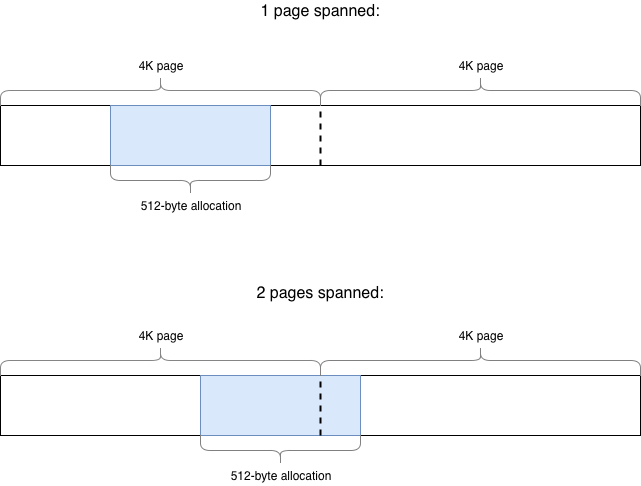
\includegraphics[width=\textwidth]{diagrams/allocation_spanned_pages.png}
	\label{fig:allocation-spanned-pages}
	\caption{A memory allocation can span different number of pages depending on where it begins}
\end{figure}

\subsection{Handling realloc}
\todo{Is this interesting to write about? It's just a software engineering problem, nothing theoretically interesting about it}

%The standard \lstinline!realloc()! function has more complicated behaviour. For instance, \lstinline!realloc(NULL, some_size)! is valid and equivalent to calling \lstinline!malloc(some_size)! in order to simplify user code. Next, Dangless needs to be able the cases both when the original came from Dangless (so is a remapped pointer), and when it did not. For instance, it's possible that the original pointer came from an allocation before Dangless finished initializing, or was created when Dangless did not have available virtual memory to perform remapping.
%
%In order to determine whether the original pointer was remapped or not, we use the same logic as during \lstinline!dangless_free()!: perform a page-table walk to get the backing physical address and then check whether the received pointer is one that would be generated by Dune when mapping its memory layout by checking the result of \lstinline!dune_pa_to_va()!. If we find that it's not a remapped pointer, then for the purposes of Dangless, this is a new allocation: simply forward the call to \lstinline!sysrealloc()! and remap the resulting pointer.
%
%Otherwise, the situation is more complicated. We have to handle the case when \lstinline!sysrealloc()! performed an in-place resize.

\section{Fixing up vmcalls}
\label{sec:vmcall-pointer-rewriting}

\subsection{The problem}

One of the goals of Dune is to remain as simple as possible, and not re-implement most functionality of operating system kernels when not absolutely necessary. This means that most system calls performed the application running inside Dune are not actually handled by Dune itself, but rather are passed on to the host kernel via the \lstinline!vmcall! instruction. (\lstinline!vmcall! is identical to \lstinline!syscall!, except it exits the virtual environment first.) This includes tasks as common as I/O operations (such as \lstinline!printf()! or \lstinline!fopen()!), or even memory management (such as \lstinline!mmap()!).

This presents a challenge for Dangless, which can be efficient because it can directly manipulate the page tables inside the virtual environment (guest machine) itself, without having to manipulate the host's page tables (which would only be possible via a system call such as \lstinline!mprotect()!). However, any virtual memory addresses returned from Dangless will only be valid inside the guest environment, meaning that attempting to pass such a memory address to the host kernel when performing a system call (vmcall) will fail with \lstinline!EINVAL!.

To demonstrate the problem, first consider the following:

\begin{lstlisting}
puts("Hello world!\n");
\end{lstlisting}

The \lstinline!puts()! standard library function used here is a comparatively simple wrapper around the \lstinline!write()! system call, and unlike \lstinline!printf()!, does not perform any formatting or other manipulation of the string~\cite{glibc-puts-analysis}. Recall that in C, strings are represented by null-terminated character arrays, and are typically passed to functions as \lstinline!const char*!: a (virtual) memory address pointing to the first character of the string. Since in this example, the argument to \lstinline!puts()! is a string literal, the string data is stored in the executable's data section (such as \texttt{.rodata}) without any dynamic memory allocation that would go through Dangless. The result is that the pointer passed to the \lstinline!write()! vmcall references virtual memory that is mapped by the host machine, so the call will succeed.

\begin{lstlisting}
void determineAnswer(char* buffer) {
	strcpy(buffer, "Fourty-two");
}

char* answerBuffer = malloc(64 * sizeof(char));
determineAnswer(answerBuffer);

puts("The answer is: ");
puts(answerBuffer);
puts("\n");

free(answerBuffer);
\end{lstlisting}

I hope that the problem is now clear: we're passing a \lstinline!malloc()!-d buffer to \lstinline!puts()!. Since \lstinline!malloc()! refers to \lstinline!dangless_malloc()!, it will perform virtual memory remapping inside the guest system, yielding a pointer value in \lstinline!answer! that is valid inside the guest machine, but not in the host machine. (Of course, the data is present in the host physical memory, but is not mapped to host virtual memory.) The \lstinline!write()! system call when executed by the host, is not going to be amused by this fact, and is going to return the error code \texttt{EINVAL}, indicating an invalid argument.

In this case by knowing how Dangless works it is easy to spot the problem. However, often dynamic memory allocation is performed and the resulting pointer is passed to a system call in a way that's not immediately obvious from the user code, such as when done internally by the standard library implementation. The simplest example is probably \lstinline!printf()!, which can call \lstinline!malloc()! in some circumstances~\cite{glibc-printf-malloc}~\cite{glibc-printf-malloc-vulnerability}. I've also already mentioned how \lstinline!dlsym()! when running for the first time will call \lstinline!calloc()!.

\subsection{Intercepting vmcalls}

In order to fix this problem, Dangless needs to intercept any system calls that are about to be forwarded to the host kernel. This capability is not provided by default in Dune, so I've implemented it (\texttt{dune-ix-vmcallhooks.patch}), allowing Dangless to register a pre- and post-hook function that will be called before and after a \lstinline!vmcall! instruction is performed by Dune, respectively. In the pre-hook, Dangless can access and modify the system call number, any of the arguments, and even the return address. Similarly, the post-hook exposes the syscall return code.

\subsection{Determining which arguments to rewrite}

The next problem is how to determine what the system call arguments are, and which of them can possibly reference a Dangless-remapped pointer. Note that it is not sufficient to find the pointers among the arguments themselves, as pointers can be nested: the arguments can be pointers to arrays or structures which in turn contain pointers -- sometimes, after a few layers of indirection. Examples include the \lstinline!readv()! and \lstinline!writev()! system calls, which are used by GNU implementation of the \lstinline!<iostream>! standard C++ header such as when writing to \lstinline!std::cout!, i.e. \lstinline!stdout!:

\begin{lstlisting}
ssize_t readv (int fd, const struct iovec *v, int n);
ssize_t writev(int fd, const struct iovec *v, int n);

struct iovec {
	void  *iov_base; /* Starting address */
	size_t iov_len;    /* Number of bytes */
};
\end{lstlisting}

When handling either of these functions, not just the \lstinline!const struct iovec *v! pointer has to be fixed, but also the \lstinline!void *iov_base! pointer inside the pointer \lstinline!struct iovec!.

Another example is the functions \lstinline!execve()! and \lstinline!execveat()!:

\begin{lstlisting}
int execve(const char *filename, char *const argv[], char *const envp[]);
int execveat(int dirfd, const char *pathname, char *const argv[], char *const envp[], int flags);
\end{lstlisting}

Besides the \lstinline!const char *filename! simple pointer, the parameters \lstinline!char *const argv[]! and \lstinline!char *const envp[]! are both a null-terminated array of pointers, in which every entry has to be fixed.

Finally, pointers to more complicated structures are also sometimes passed as system call arguments:

\begin{lstlisting}
ssize_t recvmsg(int sockfd, struct msghdr *msg, int flags);

struct msghdr {
	void         *msg_name;       /* optional address */
	socklen_t     msg_namelen;    /* size of address */
	struct iovec *msg_iov;        /* scatter/gather array */
	size_t        msg_iovlen;     /* # elements in msg_iov */
	void         *msg_control;    /* ancillary data, see below */
	size_t        msg_controllen; /* ancillary data buffer len */
	int           msg_flags;      /* flags on received message */
};
\end{lstlisting}

So, we need some way to determine which arguments of the system call can be a pointer, and identify what data structure it points to in order to find any nested pointers. Essentially, what we need is to be able to tell for a system call number what arguments it takes and what type they are. For this purpose, I have created a Python module \texttt{linux-syscallmd} (source on GitHub~\cite{github-linux-syscallmd}) that parses the Linux kernel header file \texttt{include/linux/syscalls.h} and exposes system call metadata to user code. The Dangless script at \texttt{make/gen\_vmcall\_fixup\_info.py} then uses this information to generate a file containing C code that can be \lstinline!#include!-d to utilize this data inside Dangless:

\begin{lstlisting}
// sources/src/platform/dune/vmcall_fixup_info.h

enum vmcall_param_fixup_type {
	VMCALL_PARAM_NONE,
	VMCALL_PARAM_FLAT_PTR,
	VMCALL_PARAM_IOVEC,
	VMCALL_PARAM_PTR_PTR,
	VMCALL_PARAM_MSGHDR
}

struct vmcall_param_fixup_info {
	enum vmcall_param_fixup_type fixup_type;
};

struct vmcall_fixup_info {
	i8 num_params;
	struct vmcall_param_fixup_info params[SYSCALL_MAX_ARGS];
};

// sources/src/platform/dune/vmcall_fixup_info.c

static const struct vmcall_fixup_info g_vmcall_fixup_info_table[] = {
	// generated by make/gen_vmcall_fixup_info.py
	#include "dangless/build/common/vmcall_fixup_info.inc"
};
\end{lstlisting}

The generated array is indexed by the number of a system call to find its corresponding entry. Then we can iterate through the arguments and act on them based on the \lstinline!enum vmcall_param_fixup_type! value.

As an example, the entry for the \lstinline!clone()! system call looks like this:

\begin{lstlisting}
static const struct vmcall_fixup_info s_clone_info = {
	.num_params = 5,
	.params = {
		// unsigned long flags
		[0] = {
			.fixup_type = VMCALL_PARAM_NONE
		},
		
		// void *child_stack
		[1] = {
			.fixup_type = VMCALL_PARAM_FLAT_PTR
		},
		
		// int *ptid
		[2] = {
			.fixup_type = VMCALL_PARAM_FLAT_PTR
		},
		
		// int *ctid
		[3] = {
			.fixup_type = VMCALL_PARAM_FLAT_PTR
		},
		
		// unsigned long newtls
		[4] = {
			.fixup_type = VMCALL_PARAM_NONE
		}
	}
};
\end{lstlisting}

\subsection{Rewriting the pointers}

Now that we know which arguments to rewrite or "fix-up", we can use the same logic as \lstinline!dangless_free()! to get the canonical pointer from a potentially-remapped one (see Section~\ref{ssec:deallocations}). We then replace the remapped pointer value with the canonical one in the system call arguments.

In case of nested pointers this involves modifying the referenced in-memory data, meaning we cannot simply replace the pointer. This is because the original pointer was a remapped pointer, allocated via Dangless, and will be deallocated via Dangless. However, due to the nested pointer fix-up, the user code can now potentially access the canonical (non-remapped) pointer, opening the door to dangling pointer errors. Furthermore, should a canonical pointer be passed to \lstinline!dangless_free()!, it cannot invalidate the remapped memory region as it doesn't know where it might be.

To demonstrate, consider the following code:

\begin{lstlisting}
char *first = malloc(32);
strcpy(first, "Hello ");

char *second = malloc(32);
strcpy(second, "world!");

struct iovec iov[2];
iov[0].iov_base = first;
iov[0].iov_len = strlen(first);
iov[1].iov_base = second;
iov[1].iov_len = strlen(second);

writev(STDOUT_FILENO, iov, 2);
\end{lstlisting}

Due to pointer rewriting the system call succeeds, but afterwards we end up with \lstinline|iov[0].iov_base != first| and \lstinline|iov[1].iov_base != second|, as they have been replaced by their canonical counterparts to make the system call succeed on the host kernel.

Later, we deallocate the buffers:

\begin{lstlisting}
free(second);
free(first);
\end{lstlisting}

This is fine, since the \lstinline!first! and \lstinline!second! variables were not affected by the pointer rewriting, so Dangless correctly invalidates the remapped regions in \lstinline!dangless_free()!. But then, later:

\begin{lstlisting}
fprintf(stderr, "Attempted writev() with '%s' and '%s'!\n", iov[0].iov_base, iov[1].iov_base);
\end{lstlisting}

Here we have an attempted memory access through two dangling pointers. Recall that, due to pointer rewriting, \lstinline|iov[0].iov_base| and \lstinline|iov[1].iov_base| are the canonical pointers (as returned by \lstinline!sysmalloc()!) and so do not point into the remapped region that was invalidated by the earlier \lstinline!dangless_free()! calls. Therefore, this error will not be caught by Dangless!

To resolve this situation, for every nested pointer fix-up, Dangless records the pointer location (a pointer to the user pointer) as well as the original value stored there (the Dangless-remapped pointer value) in a buffer. After the vmcall returns but before it jumps back into user code, we then go through the records and restore any such rewritten pointer values to their original ones, preventing the user from being exposed to non-remapped pointer values.

\subsection{Limitations}

This approach is limited in that Dangless can only handle system calls, arguments, and argument types that \texttt{linux-syscallmd} recognizes when building Dangless.

For instance, \texttt{linux-syscallmd} currently does not understand or process preprocessor macros, such as \lstinline!#if! and \lstinline!#ifdef! sections. This means that system call signatures not relevant for the current system will also be parsed, leading to conflicting signatures for some system calls, such as \lstinline!clone()!. \texttt{linux-syscallmd} currently does not handle this situation, and will just pick the last occurrence of the same system call in the source file, which may be different than the signature actually used by the kernel. Because of this, Dangless has special handling of the \lstinline!clone()! system call, but naturally that can't extend to e.g. system calls introduced in the future.

As of writing, I do not know of a better way to approach this. Fixing the present limitation would involve knowing what values were used for each preprocessor macro while building the kernel, and I'm not aware of any way in which the kernel exposes this information.

Another issue is understanding which arguments can hold pointer or nested pointer values. For the vast majority of system calls this is straight-forward, as \texttt{linux/syscall.h} consistently marks the pointer arguments as \lstinline!__user *!, and the pointed type is obvious, whether it's \lstinline!char! or \lstinline!struct iovec!. But some system calls will interpret the same argument differently depending on the context of the call, such as \lstinline!ptrace()!. The signature of \lstinline!ptrade()! is as follows:

\begin{lstlisting}
long ptrace(enum __ptrace_request request, pid_t pid, void *addr, void *data);
\end{lstlisting}

Notice that \lstinline!addr! and \lstinline!data! are both untyped (\lstinline!void!) pointers. How they are interpreted differs depending on the value of the \lstinline!request! argument. Some examples:

\begin{itemize}
	\item \lstinline!PTRACE_TRACEME!: both \lstinline!addr! and \lstinline!data! are ignored.
	\item \lstinline!PTRACE_PEEKTEXT!: \lstinline!addr! does \emph{not} correspond to pointer in the address space of the caller, but rather, refers to a location in the address space of the target application. The same pointer value may reference a memory region that's unmapped, or worse, mapped for something completely different in the address space of the calling process. As such, Dangless should not touch it. \lstinline!data! is ignored.
	\item \lstinline!PTRACE_POKEDATA!: \lstinline!addr! refers to a memory address in the target process. \lstinline!data! might not be a pointer value at all, but rather the word to be copied into the target process' memory.
	\item \lstinline!PTRACE_GETREGS!: \lstinline!data! is an actual pointer in the calling process, while \lstinline!addr! is ignored.
	\item \lstinline!PTRACE_GETREGSET!: \lstinline!addr! is not a pointer value at all, but rather an enumeration. \lstinline!data! is an actual pointer to the calling process' memory, but it references a \lstinline!struct iovec! value, meaning that it will contain nested pointers that also have to be fixed up by Dangless.
\end{itemize}

\lstinline!ptrace()! is a special case due to its very specialized nature, and it's unlikely to be used at all in the vast majority of applications that Dangless would be relevant for. Because of this Dangless ignores \lstinline!ptrace()!, even though it would be possible to cover all of these scenarios.

There may be other system calls that have similar behaviour, although likely not as pathological as \lstinline!ptrace()!. These are currently not handled in any way by texttt{linux-syscallmd} nor Dangless. Supporting all of these scenarios would inevitably involve extending Dangless to handle each on a case-by-case basis.

\todo{Probably have a chapter about using Dangless, such as how to build Dangless, what system requirements does it have, and how to make it work on an existing application.}
